\documentclass{beamer}
\usepackage[utf8]{inputenc}
\usepackage{hyperref}
\usepackage{multicol}
\usepackage{hyperref}
\usepackage{amsmath}
\usepackage[english]{babel}
\usepackage{algorithm}
\usepackage[noend]{algpseudocode}

\inputencoding{utf8}

\mode<presentation> {
    \usetheme{Madrid}
}

\usepackage{graphicx}
\usepackage{booktabs}

\title[Tiempo Lineal]{Ordenamiento en tiempo lineal}
\author{Ernesto Rodriguez - Juan Roberto Alvaro Saravia}
\institute{
    Universidad Francisco Marroquin \\
    \medskip \textit{ernestorodriguez@ufm.edu - juanalvarado@ufm.edu}
}

\date[\today]{}

\begin{document}

\begin{frame}
\titlepage
\end{frame}


\begin{frame}
    \frametitle{Algoritmos de Comparaci\'on}
    \begin{itemize}
        \item{Funciona mediante la comparaci\'on directa
            entre parejas de elementos.}
        \item{Los elementos se pueden comparar mediante cualquier
            criterio, siempre y cuando dicho criterio sea un \emph{orden total}}
        \item{Todos los algoritmos estudiados hasta el momento son
            \emph{Algoritmos de Comparaci\'on}}
        \item{Los \emph{Algoritmos de Comparaci\'on} tienen un rendimiento
        maximo de $\mathcal{O}(nlog(n))$}

    \end{itemize}
\end{frame}

\begin{frame}
    \frametitle{Rendimiento de Algoritmos de Comparaci\'on}
    Premisas:
    \begin{itemize}
        \item{Solo es posible obtener informaci\'on sobre los elementos
        mediante comparaci\'on directa.}
        \item{Todos los elementos son diferentes (simplifica el analisis)}
        \item{No existe informaci\'on posicional absoluta de los elementos,
        solo relativa a otros elementos.}
        \item{Las distintas comparaciones possibles $<,\leq,>,\geq,\mathtt{ect}$ forman
        ordenes, por lo cual todas son equivalentes a $\leq$}
    \end{itemize}
\end{frame}

\begin{frame}
    \frametitle{Arboles de Decisi\'on}
    \begin{itemize}
        \item{Modelan la ejecuci\'on de un \emph{Algoritmo de Comparaci\'on}}
        \item{Cada hoja representa una permutaci\'on de
            la entrada (por lo que hay $n!$ hojas)}
        \item{El camino de la raiz hacia una hoja representa las comparaciones
        que se llevan a cabo para escoger dicha permutaci\'on}
        \item{Todo algoritmo de ordenamiento debe escoger alguna permutaci\'on
        de la entrada como respuesta.}
    \end{itemize}
\end{frame}

\begin{frame}
    \frametitle{Arboles de Desici\'on}
    \begin{center}
        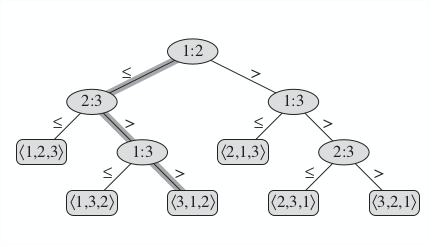
\includegraphics[width=8cm]{./cmpTree.png}
    \end{center}
    Ejecuci\'on del algoritmo con [6,8,5] de entrada.
\end{frame}

\begin{frame}
    \frametitle{Arbol de Desici\'on}
    \begin{itemize}
        \item{Todas las permutaciones de la entrada deben ser accesibles
        por el \emph{arbol de desici\'on}}
        \item{Alcanzar una permutaci\'on require que se recorra un camino
        en el arbol de desici\'on.}
        \item{Por lo cual la altura de dicho arbol corresponde a la peor
        ejecuci\'on possible}
        \item{Un \emph{Algoritmo de Comapraci\'on} tiene una ejecuci\'on limitada
        por la altura del \emph{arbol de desici\'on.}}
        \item{Eso significa que el peor de los casos requiere $log(n!)$ comparaci\'ones, pero
        $log(n!)\in \mathcal{O}(nlog(n))$}
    \end{itemize}
\end{frame}


\end{document}